\chapter{Caracteristicas de transferencia de Corriente}
  Las \textbf{características de transferencia de corriente} del transistor BJT describen la relación entre la corriente
  de base $I_B$ y la corriente de colector $I_C$, manteniendo constante la tensión colector-emisor $V_{CE}$. Esta
  relación es clave en la región activa del transistor, donde éste funciona como amplificador de corriente.

  En dicha región, se cumple la relación:

  \begin{equation}
    I_C = \beta \cdot I_B
  \end{equation}

  donde $\beta$ (también conocido como $h_{FE}$) representa la ganancia de corriente continua del transistor en
  configuración emisor común. Esta relación es aproximadamente lineal para un amplio rango de operación y es la base del
  comportamiento amplificador del BJT.
  
  El estudio experimental de estas características permite determinar el valor de $\beta$ y observar cómo varía con
  $I_B$, facilitando la comprensión del funcionamiento interno del transistor y su comparación con el modelo teórico.

  \section{Simulacion}

    En esta etapa se realiza la simulación del circuito para obtener la curva $I_C$ vs.\ $I_B$, con $V_{CE}$ constante.
    Se utiliza una barrida de corriente de base para analizar el comportamiento del transistor y estimar su ganancia de
    corriente continua $\beta$.

    \begin{figure}[!ht]
      \centering
      \begin{minipage}{0.45\textwidth}
        \begin{tikzpicture}[circuitikz, straight voltages]
          % Paths, nodes and wires:
          \draw node[npn] (N1) at (8, 6.23) {} node[anchor=west] at (N1.text){$BC547B$};
          \draw (7.16, 6.23) to[american resistor, l={$100K \, \Omega$}, label distance=0.02cm] (5, 6.23);
          \draw (8.5, 7.75) to[american resistor, l={$560 \, \Omega$}, label distance=0.02cm] (10.5, 7.75);
          \draw (8, 7) -| (8, 7.75);
          \draw (11, 6.75) to[battery, l={$V_{CC}$}, label distance=0.02cm] (11, 5.75);
          \draw (11, 6.75) -| (11, 7.75);
          \draw (8, 5.46) -- (8, 4);
          \draw (11, 5.75) -- (11, 4);
          \draw node[ground] at (8, 4) {};
          \draw node[ground] at (11, 4) {};
          \draw (8, 7.75) -- (8.5, 7.75);
          \draw (10.5, 7.75) -- (11, 7.75);
          \draw (5, 5.5) to[battery, l={$V_{BB}$}, label distance=0.02cm] (5, 4.5);
          \draw (5, 5.5) |- (5, 6.23);
          \draw (5, 4.5) -| (5, 4);
          \draw node[ground] at (5, 4) {};
        \end{tikzpicture}
        \caption{Circuito de prueba para polarizacion.}
        \label{crkt:corr}
      \end{minipage}
      \hfill
      \begin{minipage}{0.45\textwidth}
        \begin{lstlisting}[style=ltspice, caption={Parámetros de simulación LTspice}, label=list:corr]
.dc VBB 0 5 200m
.step param VCC list 2 5 10
        \end{lstlisting}
      \end{minipage}
    \end{figure}

    \begin{figure}[H]
      \centering
      \includegraphics[width=1\textwidth]{images/graph_ib_ic.png}
      \caption{Grafico de corriente del colector respecto a la corriente de base.}
    \end{figure}

  \section{Laboratorio}

    Se realizan mediciones experimentales de $I_C$ en función de $I_B$ con tensión $V_{CE}$ fija, replicando condiciones
    similares a las de la simulación. Esto permite comparar el modelo teórico del BJT con su comportamiento real en
    laboratorio.

    Debido a que el circuito a analizar es el mismo que el ejercicio anteror, puede revisar las configuraciones del
    multimetro mostradas previamente.

    Se presenta el cuadro con las medidas obtenidas:

    \begin{table}[h!]
      \centering
      \begin{tabular}{|c|c|c|c|}
        \hline
        $I_B$ [$\mu$A] & $I_C$ ($V_{CE} = 2\,V$) & $I_C$ ($V_{CE} = 5\,V$) & $I_C$ ($V_{CE} = 8\,V$) \\ \hline
        5  & $1.56 \, mA$ & $1.78 \, mA$  & $1.71 \, mA$ \\ \hline
        7  & $1.72 \, mA$ & $2.32 \, mA$  & $2.42 \, mA$ \\ \hline
        10 & $3.49 \, mA$ & $3.42 \, mA$  & $3.51 \, mA$ \\ \hline
        20 & $6 \, mA$    & $6.85 \, mA$  & $7.14 \, mA$ \\ \hline
      \end{tabular}
      \caption{Corriente de colector medida para distintos valores de $V_{CE}$ e $I_B$ constantes.}
    \end{table}
    
    \begin{figure}[H]
      \centering
      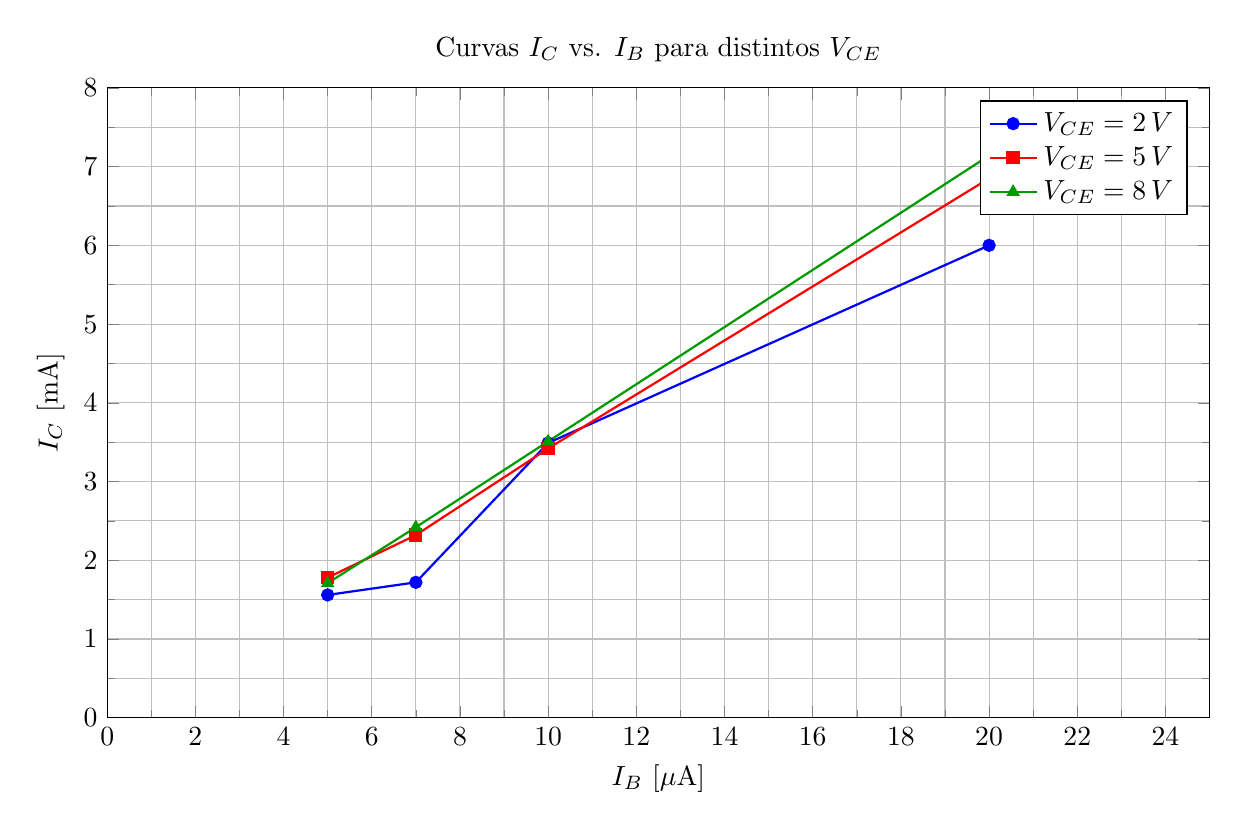
\begin{tikzpicture}
        \begin{axis}[
          width=14cm,
          height=8cm,
          xlabel={$I_B$ [$\mu$A]},
          ylabel={$I_C$ [mA]},
          grid=both,
          minor tick num=1,
          scale only axis,
          enlargelimits=false,
          title={Curvas $I_C$ vs. $I_B$ para distintos $V_{CE}$},
          scaled ticks=false,
          xmin=0, xmax=25,
          ymin=0, ymax=8
        ]
      
        % V_CE = 2 V
        \addplot[
          mark=*,
          color=blue,
          thick
        ] coordinates {
          (5, 1.56)
          (7, 1.72)
          (10, 3.49)
          (20, 6)
        };
        \addlegendentry{$V_{CE} = 2\,V$}
      
        % V_CE = 5 V
        \addplot[
          mark=square*,
          color=red,
          thick
        ] coordinates {
          (5, 1.78)
          (7, 2.32)
          (10, 3.42)
          (20, 6.85)
        };
        \addlegendentry{$V_{CE} = 5\,V$}
      
        % V_CE = 8 V
        \addplot[
          mark=triangle*,
          color=green!60!black,
          thick
        ] coordinates {
          (5, 1.71)
          (7, 2.42)
          (10, 3.51)
          (20, 7.14)
        };
        \addlegendentry{$V_{CE} = 8\,V$}
      
        \end{axis}
      \end{tikzpicture}
    \end{figure}


  A lo largo de esta experiencia, realizamos la medición de las curvas características del transistor, obteniendo datos
  experimentales de $I_C$ en función de $V_{CE}$ para distintos valores de $I_B$. Posteriormente, representamos
  gráficamente las curvas tanto a partir de los datos medidos como de las simulaciones. Estas representaciones nos
  permitieron identificar las distintas regiones de operación del transistor (corte, activa y saturación), y analizar su
  comportamiento ante variaciones en la corriente de base.

  Sin embargo, al comparar las gráficas simuladas con las obtenidas experimentalmente, nos dimos cuenta de un error
  metodológico en el proceso de medición: cada vez que cambiábamos $I_B$, también ajustábamos manualmente el valor de
  $V_{CE}$, cuando en realidad lo correcto habría sido fijar inicialmente $V_{CE}$ (por ejemplo, para $I_B = 0$) y luego
  permitir que este variara naturalmente a medida que cambiaba $I_B$. Esta equivocación afectó la fidelidad de los datos
  registrados y generó discrepancias respecto al comportamiento ideal del transistor. Este análisis nos permitió
  entender mejor la importancia de mantener condiciones controladas y consistentes en la caracterización de dispositivos
  electrónicos.
